\section{Test setting}

The subject will be placed in a upholstered chair with adjustable backrest, footrest and armrests, which allows a good positioning of the measured hand, while the subject remain in a relaxed position. Measurement will be carried out on the dominant hand. The hand is stabilized with a vacuum pillow which is covered by a micro fiber tissue to get a better background for the images. Microfiber has a low heat conduction \cite{schacher2000}. That helps to identify the outlines of the hand on the thermal image, because the tissue is not conducting the temperature of the hand to a high extent. To provide a more comfortable position of the arm during the experiment the armrest of the adjustable chair is padded with some sheets under the vacuum pillow. A comfortable position in the chair is important, because the subject has to sit still and is not allowed to move during the test for at least 45 min. These precautions only counteract some small movement, and therefore it is important that the subject is focused on sitting still. 
$37,5\pm 1,0$ cm over the hand the Gobi $640$ $17\mu$m GigE infrared camera (Xenics NV, Belgium) is positioned with a tripod. The setup with camera, chair and computer can be seen on \figref{fig:setting}. 


\begin{figure}[H]
	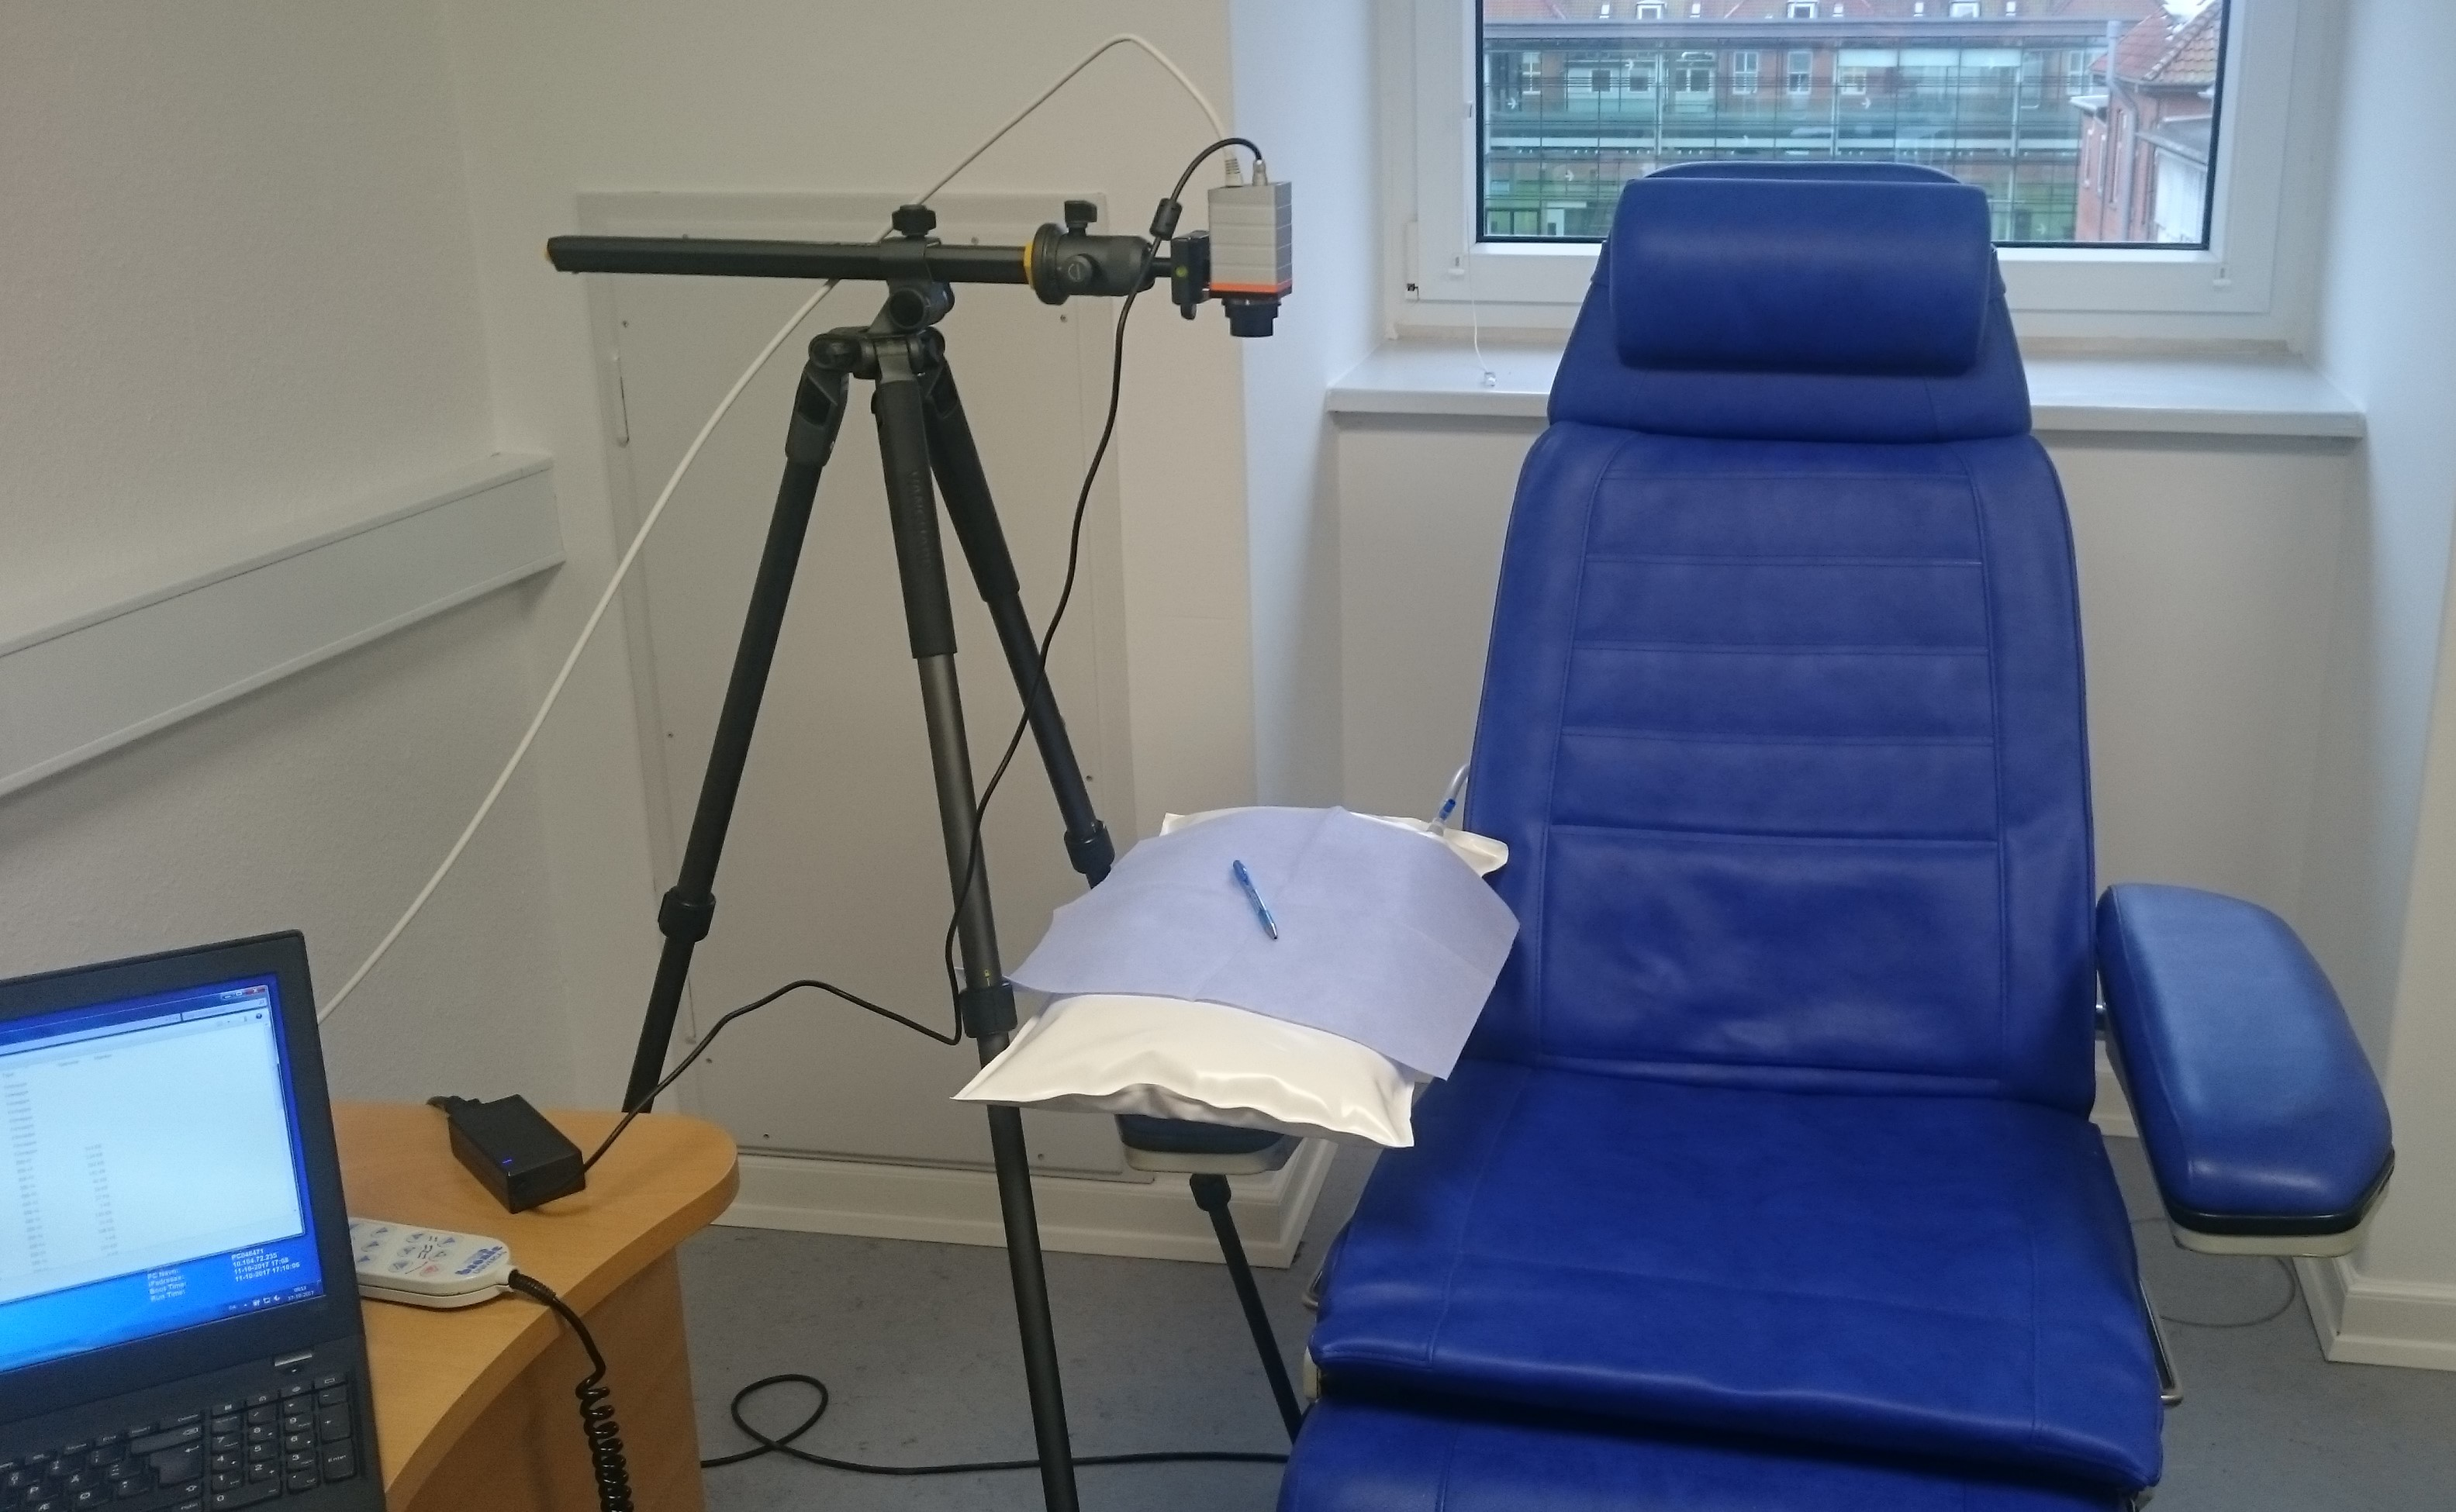
\includegraphics[width=0.7\textwidth]{figures/setting}
	\caption{The test setting at the Regionshospital Nordjylland.}
	\label{fig:setting}
\end{figure}

The camera is via a Ethernet cable connected with a laptop, which is used to record the measurements with Xeneth 2.6 software. 
First cable connections between the camera, the laptop and the power supply have to be set. Afterwards the camera is turned on and has to warm up for about 15 min. During this the laptop should be started and the software for taking the measurements is set in operational readiness.

When the preparation of the test setting is done, the preparation for the subject can begin. At first the blood pressure of the subject is measured on the dominant arm. The blood pressure is measured three times while the subject is sitting relaxed on a chair. Mean systolic blood pressures is calculated. To get the total occlusion pressure $(TOP)$ the mean has to be multiplied by 1.3. To reduce the blood flow in the arm to 50\% during the measurement within the second condition, the arm is cuffed with 30\% of the $TOP$.\cite{mouser2017} 
The cuff is then affixed at the subjects dominant arm without tighten it, so that it is ready for the second part of the experiment. After that the subject can take place in the chair and the hand can be stabled with the vacuum pillow. The vacuum generator is attached to the pillow for giving the hand more stability. The lens focus has to be adjusted so the distance is taking in to consideration, to make sure the image is sharp.

If the camera is stable and the filename is modified according to the subject, the first measurement can be started for 20 min. The time needs to be measured by a stopwatch. During the whole experiment the subject is not allowed to move or speak to minimize movement bias.
Directly after the first measurement the cuff on the arm of the subject is tightened with the calculated value. The pressure of the cuff should be observed during the whole measurement and if necessary adjusted.

To guide the conductors of the experiment, an experimental protocol has been formed and to be followed during the experiment. The experimental protocol can be seen in \cref{chap:protocol}. 

